\chapter{Inflation durch ein rollendes Skalarfeld}

\lectureoverview{Eine aus der vorherigen Sitzung offen gebliebene Frage gibt die leitende Gleichung vor,
\(\ddot\phi+3H\dot\phi=-V'(\phi)\): Was bewegt sich, was übt die Kraft aus, und warum ähnelt die Expansion einer Reibung? Wir leiten die Gleichung zunächst in einer festen Box und dann in einer expandierenden her. Koppelt man sie an die Friedmann-Gleichung, ergibt sich der Slow-Roll-Mechanismus: Ein hohes, flaches Skalarpotential treibt eine nahezu exponentielle Expansion an. Die Inflation verdünnt Monopole und glättet die Geometrie; ihr Ende heizt das Universum wieder auf und leitet den konventionellen heißen Urknall ein. Damit stellt sich unweigerlich die letzte Frage: Wenn die Inflation so effizient glättet, woher stammt dann die Struktur? Eine eindimensionale Kaustikrechnung zeigt, wie winzige Geschwindigkeitsunterschiede Schichten, Filamente und Knoten erzeugen, während der quantenmechanische Ursprung dieser Unterschiede der nächsten Vorlesung vorbehalten bleibt.}

\section{Worauf wirkt was?}

Die Eingangsfrage greift die Gleichung
\begin{equation}
\ddot\phi+3H\dot\phi
=F(\phi)
=-\frac{dV}{d\phi}
\label{eq:c09-opening}
\end{equation}auf und fragt, welche Art von Kraft \(F\) auf ein Feld wirken kann. Diese Frage ist keineswegs nebensächlich. Um sie zu beantworten, müssen wir die Mechanik des Feldes rekonstruieren und beginnen damit zugleich, das Inflationsthema selbst zu behandeln.

Ein Skalarfeld ordnet jedem Punkt in Raum und Zeit eine Zahl \(\phi(\mathbf x,t)\) zu. Elektrische und magnetische Felder tragen Energie; auch ein Skalarfeld kann Energie tragen. Das hier benötigte Feld ist hypothetisch: Es wurde kein bestimmtes Inflaton experimentell identifiziert, daher ist seine Energie als Funktion des Feldwerts unbekannt. Wir stellen sie deshalb durch eine nicht näher spezifizierte potentielle Energiedichte dar:
\begin{equation}
V=V(\phi).
\label{eq:c09-potential}
\end{equation}
Verschiedene Werte von \(\phi\) entsprechen unterschiedlichen Energiemengen, die pro Einheit des physikalischen Volumens gespeichert sind.

Es gibt keinen Grund dafür, dass \(\phi=0\) energiefrei sein muss. Der Ursprung des Feldraums ist Konvention, insbesondere bei einem noch unentdeckten Feld; eine Verschiebung der Koordinate, mit der Feldwerte bezeichnet werden, muss das Minimum von \(V\) nicht in den Ursprung legen. Der Graph von \(V(\phi)\) beschreibt relative Steigungen und Höhen, aber keinen ausgezeichneten Ausgangspunkt des Feldes.

Die potentielle Energie ist der Anteil, der verbleibt, wenn das Feld momentan statisch ist. Ändert sich das Feld mit der Zeit, besitzt es zusätzlich kinetische Energie. Die Größe \(\dot\phi\) ist nicht die Geschwindigkeit eines Objekts durch den gewöhnlichen Raum, sondern die Änderungsrate des Feldwerts, also eine Geschwindigkeit im Feldraum. Eine elastische Saite bietet eine nützliche Analogie. Ihre Auslenkung ist ein Feld auf einer eindimensionalen Welt, und ein schwingendes Saitenelement trägt kinetische Energie, die proportional zum Quadrat seiner zeitlichen Ableitung ist.

Der Vorfaktor dieses Quadrats lässt sich in die Definition des Feldes aufnehmen. Beginnt man mit
\begin{equation}
\frac12 n^2\dot\phi^{\,2},
\end{equation}
so verwandelt die Variablentransformation
\begin{equation}
\chi=n\phi
\end{equation}
den Term in \(\dot\chi^{\,2}/2\). Wir können daher ein kanonisch normiertes Feld wählen und in der homogenen Näherung schreiben:
\begin{equation}
\rho_\phi=\frac12\dot\phi^{\,2}+V(\phi).
\label{eq:c09-rho-homogeneous}
\end{equation}
Diese Wahl normiert die Koordinate im Feldraum; sie bedeutet nicht, dass eine tatsächliche Teilchenmasse gleich eins gesetzt wurde.

\section{Mechanik in einer festen Box}

Betrachten wir eine kleine Box, in der das Feld räumlich nahezu konstant ist. Ihre Energiedichte hat dieselbe mathematische Form wie die Energie eines Teilchens der Masse eins: kinetischer plus potentieller Anteil. Die zugehörige Lagrangedichte hat beim Potential das entgegengesetzte Vorzeichen:
\begin{equation}
\mathcal L_\phi
=\frac12\dot\phi^{\,2}-V(\phi).
\label{eq:c09-lagrangian-density}
\end{equation}
Die Analogie ist mathematischer Art. Die verallgemeinerte Koordinate ist der Feldwert, nicht die räumliche Position eines Teilchens.

Die Euler---Lagrange-Gleichung lautet:
\begin{equation}
\frac{d}{dt}
\left(
\frac{\partial\mathcal L_\phi}{\partial\dot\phi}
\right)
=
\frac{\partial\mathcal L_\phi}{\partial\phi}.
\label{eq:c09-el-fixed}
\end{equation}
Hier ist die Geschwindigkeitsvariable \(\dot\phi\), also gilt
\begin{equation}
\frac{\partial\mathcal L_\phi}{\partial\dot\phi}=\dot\phi,
\qquad
\frac{\partial\mathcal L_\phi}{\partial\phi}=-V'(\phi),
\end{equation}
und damit erhalten wir
\begin{equation}
\ddot\phi=-V'(\phi)\equiv F(\phi).
\label{eq:c09-fixed-eom}
\end{equation}
Die zweite Ableitung ist die Beschleunigung der Feldkoordinate, und die negative Steigung des Potentials ist ihre Kraft.

\begin{figure}[htbp]
\centering
\includegraphics[width=0.88\textwidth]{lecture_09_figure_03.png}
\caption{Der lesbare Teil der Tafel zeigt \(V(\phi)\) und die Gleichung für die feste Box \(\ddot\phi=-\partial V/\partial\phi\). Der obere Euler---Lagrange-Ausdruck ist teilweise abgeschnitten und verdeckt. Gleichung~\eqref{eq:c09-el-fixed} wurde daher aus der Herleitung rekonstruiert und nicht als vollständig sichtbare Tafelaufschrift wiedergegeben.}
\label{fig:c09-fixed-board}
\lectureframe{00:10:53.836}
\end{figure}

\begin{classroomqa}
\audiencequestion{Was ist die Kraft, und worauf wirkt sie?}
\lecturerresponse{Die sich entwickelnde Größe ist der Skalarwert \(\phi\). Die Größe \(-V'(\phi)\) ist eine Kraft im Feldraum: Sie beschleunigt den Feldwert in Richtung geringerer potentieller Energie, so wie \(-dV/dx\) eine Teilchenkoordinate beschleunigt. Sie ist keine neue Vektorkraft, die einen materiellen Körper durch den gewöhnlichen Raum schiebt. \lecturetimestamp{00:00:27--00:00:49; 00:10:41--00:11:29}}
\end{classroomqa}

Das vollständige Feld kann räumlich variieren. Für ein kanonisches Skalarfeld in einer räumlich flachen, expandierenden Geometrie enthält seine lokale Energiedichte
\begin{equation}
\rho_\phi
=
\frac12\dot\phi^{\,2}
+\frac{1}{2a^2}\lvert\nabla\phi\rvert^2
+V(\phi).
\label{eq:c09-rho-full}
\end{equation}
Wir lassen den Gradiententerm weg, weil die Expansion Variationen auf große Wellenlängen streckt und das Feld dadurch innerhalb der kleinen Box nahezu homogen wird. Diese Näherung ist durch die kosmologische Situation gerechtfertigt; sie bestreitet nicht, dass Skalarwellen oder räumliche Fluktuationen auftreten können.

\section{Die expandierende Box}

Die erste Herleitung beantwortet die Eingangsfrage, ist aber noch nicht die kosmologische Herleitung. Die Gleichungen ~\eqref{eq:c09-rho-homogeneous} und \eqref{eq:c09-lagrangian-density} beschreiben Dichten. Das physikalische Volumen einer Einheitsbox in komovierenden Koordinaten ist proportional zu \(a^3(t)\), daher lautet ihre Lagrange-Funktion:
\begin{equation}
L_\phi
=a^3(t)
\left[
\frac12\dot\phi^{\,2}-V(\phi)
\right].
\label{eq:c09-comoving-lagrangian}
\end{equation}
Der Faktor \(a^3\) wäre in einer statischen Box unerheblich. In der Kosmologie hängt er von der Zeit ab, und diese Abhängigkeit liefert den fehlenden Term.

\begin{figure}[htbp]
\centering
\includegraphics[width=0.88\textwidth]{lecture_09_figure_04.png}
\caption{Links ist eine handgezeichnete Potentialkurve zu sehen, rechts sind Teile der Energie- und Lagrange-Ausdrücke erkennbar. Die Kurve und der Vorzeichenwechsel sind eindeutig; die vollständige Algebra in Gleichung~\eqref{eq:c09-comoving-lagrangian} stammt aus der mündlichen Herleitung, da der Dozent einen Teil der Tafel verdeckt.}
\label{fig:c09-potential-board}
\lectureframe{00:13:26.528}
\end{figure}

Wendet man die Euler---Lagrange-Gleichung auf \(L_\phi\) an, erhält man
\begin{align}
\frac{d}{dt}\left(a^3\dot\phi\right)
&=-a^3V'(\phi), \label{eq:c09-a3-form}\\
a^3\ddot\phi+3a^2\dot a\,\dot\phi
&=-a^3V'(\phi),\\
\ddot\phi+3\frac{\dot a}{a}\dot\phi
&=-V'(\phi).
\end{align}Mit \(H=\dot a/a\) folgt
\begin{equation}
\boxed{\ddot\phi+3H\dot\phi=-V'(\phi)}.
\label{eq:c09-hubble-friction}
\end{equation}Die zu Beginn erinnerte Gleichung ist nun hergeleitet und nicht bloß in Erinnerung gerufen.

\begin{figure}[htbp]
\centering
\includegraphics[width=0.96\textwidth]{lecture_09_figure_05.png}
\caption{Links die Dynamik in der festen Box, rechts die Korrektur für die expandierende Box. Die sichtbare Tafel belegt die Folge von \(d(a^3\dot\phi)/dt\) zu den Formen \(3\dot a/a\) und \(3H\); abgeschnittene rechte Seiten werden durch Gleichung~\eqref{eq:c09-a3-form} ergänzt.}
\label{fig:c09-expanding-board}
\lectureframe{00:18:35.380}
\end{figure}

\begin{classroomqa}
\audiencequestion{Lässt sich die Kraft \(F\) anschaulicher darstellen?}
\lecturerresponse{Zeichne \(V(\phi)\) als Landschaft, deren horizontale Koordinate der Feldwert ist. Die Steigung bestimmt die Kraft \(F=-V'(\phi)\). Eine steile Abwärtsneigung erzeugt einen starken Antrieb im Feldraum, eine flache Neigung einen schwachen. Das Bild veranschaulicht die eindimensionale Feldkoordinate; es stellt keinen buchstäblichen Hügel im physikalischen Raum dar. \lecturetimestamp{00:18:26--00:19:18}}
\end{classroomqa}

\section{Hubble-Reibung und Grenzbewegung}

Bringen wir den mittleren Term in Gleichung ~\eqref{eq:c09-hubble-friction} auf die rechte Seite:
\begin{equation}
\ddot\phi=-V'(\phi)-3H\dot\phi.
\end{equation}Für ein expandierendes Universum, \(H>0\), wirkt der zweite Term der Feldgeschwindigkeit stets entgegen. Er verhält sich daher wie eine Viskosität. Ein in zähem Honig losgelassener Stein beschleunigt zunächst, doch der Widerstand nimmt mit der Geschwindigkeit zu, bis der Stein seine Grenzgeschwindigkeit erreicht. Die Eselsbrücke \emph{\(H\) für Honig}fasst die Analogie zusammen; ihren eigentlichen Gehalt liefert die Gleichung. Ändert sich \(H\) mit der kosmischen Zeit, ändert sich auch die effektive Viskosität, ähnlich wie sich gewöhnliche Viskosität mit der Temperatur ändert.

Überwiegt die Reibung gegenüber der Trägheit, gilt \(\lvert\ddot\phi\rvert\ll3H\lvert\dot\phi\rvert\), und das Feld nähert sich rasch dem Verhalten
\begin{equation}
3H\dot\phi\simeq -V'(\phi),
\qquad
\dot\phi\simeq-\frac{V'(\phi)}{3H}.
\label{eq:c09-terminal}
\end{equation}Ein flaches Potential liefert eine kleine Kraft, während ein großes \(H\) starken Widerstand bedeutet. Beide Effekte machen \(\dot\phi\) klein und führen gewöhnlich dazu, dass die kinetische Dichte \(\dot\phi^2/2\) klein gegenüber \(V\) ist.

\begin{classroomqa}
\audiencequestion{Stützt sich diese Herleitung auf das Prinzip der kleinsten Wirkung?}
\lecturerresponse{Ja. Gleichung~\eqref{eq:c09-hubble-friction} folgt aus der Extremalisierung der Wirkung, die mit Gleichung~\eqref{eq:c09-comoving-lagrangian} gebildet wird. Man kann die Feldgleichung auch als grundlegendes dynamisches Gesetz ansetzen; die Variationsherleitung erklärt jedoch genau, weshalb das expandierende Volumen den Term \(3H\dot\phi\) beiträgt. \lecturetimestamp{00:25:40--00:26:15}}
\end{classroomqa}

\begin{classroomqa}
\audiencequestion{Wenn der neue Term wie Reibung wirkt, wohin geht dann die verlorene Energie?}
\lecturerresponse{Ein echter Stein in Honig überträgt mechanische Energie in Wärme. Die kosmologische Aussage ist subtiler. Die Lagrange-Funktion der komovierenden Box hängt über \(a(t)\) explizit von der Zeit ab. Daher ist die gewöhnliche mechanische Energie dieser Box aufgrund der Zeittranslationssymmetrie nicht erhalten. Die lokale kovariante Erhaltung des Energie-Impuls-Tensors gilt weiterhin:
\[
\dot\rho_\phi+3H(\rho_\phi+p_\phi)=0,
\qquad
p_\phi=\frac12\dot\phi^{\,2}-V(\phi).
\]
Für ein homogenes Skalarfeld wird daraus \(\dot\rho_\phi=-3H\dot\phi^{\,2}\): Das Feld verrichtet Arbeit an der expandierenden Geometrie. Was scheitert, ist die naive Annahme einer global erhaltenen Energie des sich entwickelnden Universums, nicht die lokale Erhaltung des Energie-Impuls-Tensors. \lecturetimestamp{00:26:16--00:27:57}}
\end{classroomqa}

\section{Das Feld treibt die Expansion an}

Bisher hat die Expansion auf das Skalarfeld eingewirkt. Das ist nur die eine Hälfte der Rückkopplung. Die Energiedichte des Skalarfeldes bestimmt über die flache Friedmann-Gleichung auch die Expansion:
\begin{equation}
H^2=\left(\frac{\dot a}{a}\right)^2
=\frac{8\pi G}{3}\rho.
\label{eq:c09-friedmann}
\end{equation}Für ein nahezu homogenes Skalarfeld gilt
\begin{equation}
H^2
=\frac{8\pi G}{3}
\left[
\frac12\dot\phi^{\,2}+V(\phi)
\right].
\label{eq:c09-friedmann-scalar}
\end{equation}Die Expansion dämpft das Feld, und das gedämpfte Feld kann seinerseits die Energiedichte aufrechterhalten, welche die Expansion antreibt.

\begin{classroomqa}
\audiencequestion{Ist dieses hypothetische Skalarfeld das sogenannte Inflaton?}
\lecturerresponse{Ja. Der Name bezeichnet die ihm zugeschriebene Rolle: ein Skalarfeld, dessen nahezu konstante potentielle Energie die Inflation antreibt. Die Benennung des Feldes identifiziert noch nicht seine teilchenphysikalische Natur. Das konkrete Inflaton, seine Kopplungen und sogar die Frage, ob ein einziges elementares Skalarfeld diese Rolle spielte, hängen vom jeweiligen Modell ab. \lecturetimestamp{00:30:26--00:31:28}}
\end{classroomqa}

\begin{classroomqa}
\audiencequestion{Gibt es experimentelle Belege für das Inflaton?}
\lecturerresponse{Ein bestimmtes Inflatonfeld wurde im Labor nicht direkt nachgewiesen. Die Belege sind indirekt: Die Inflationsdynamik bietet einen erfolgreichen Rahmen zur Erklärung der beobachteten Flachheit und der primordialen Störungen, doch viele Potentiale können diese allgemeinen Befunde erklären. Diese indirekte Unterstützung ist von der Kenntnis der mikroskopischen Umsetzung zu unterscheiden. \lecturetimestamp{00:31:29--00:33:02}}
\end{classroomqa}

\begin{classroomqa}
\audiencequestion{Tragen alle Felder Energie, und wäre eine skalare Anregung ein Boson?}
\lecturerresponse{Physikalische Felder tragen Energie und Impuls. Die Quantisierung eines Skalarfeldes ergibt Bosonen mit Spin null. Der bei der Inflation verwendete klassische homogene Hintergrund lässt sich am besten nicht als ein gewöhnliches Teilchen vorstellen, auch wenn sich seine Schwingungen nach der Inflation in Begriffen von Inflatonquanten beschreiben lassen. \lecturetimestamp{00:33:03--00:35:20}}
\end{classroomqa}

\begin{classroomqa}
\audiencequestion{Könnte das Higgs-Feld das Inflaton sein?}
\lecturerresponse{Ein Skalarfeld ist erforderlich, daher liegt die Analogie nahe. Das beobachtete Higgs-Feld mit seinem üblichen Standardmodellpotential und seinen Kopplungen entspricht jedoch nicht automatisch dem Feld dieses einfachen Plateaus. Modelle der Higgs-Inflation ergänzen eine nichtminimale Gravitationsstruktur. Nichts in der bisherigen Argumentation identifiziert das Inflaton mit dem Higgs-Feld. \lecturetimestamp{00:35:21--00:37:11}}
\end{classroomqa}

Stellen wir uns nun vor, \(V(\phi)\) sei hoch, falle aber über ein langes Intervall nur sanft ab. Gleichung~\eqref{eq:c09-terminal} hält das Feld in langsamer Bewegung, sodass
\begin{equation}
\frac12\dot\phi^{\,2}\ll V(\phi).
\end{equation}Die Friedmann-Gleichung vereinfacht sich zu
\begin{equation}
H^2\simeq\frac{8\pi G}{3}V(\phi),
\qquad
H\simeq
\sqrt{\frac{8\pi G}{3}V(\phi)}.
\label{eq:c09-potential-dominated}
\end{equation}Die Ableitung \(V'(\phi)\) bestimmt die langsame Bewegung des Feldes; die Höhe \(V(\phi)\) bestimmt die rasche Expansion des Raums.

\begin{figure}[htbp]
\centering
\includegraphics[width=0.92\textwidth]{lecture_09_figure_06.png}
\caption{Die Friedmann-Gleichung, die Energiedichte des Skalarfeldes und der eingerahmte, vom Potential dominierte Ausdruck. Der Wurzelterm in \(V(\phi)\) ist deutlich zu erkennen; das vorangestellte \(H\simeq\) in Gleichung~\eqref{eq:c09-potential-dominated} ist die durch die mündliche Argumentation gestützte Standardvervollständigung.}
\label{fig:c09-friedmann-board}
\lectureframe{00:41:04.178}
\end{figure}

Ändert sich \(V\) nur geringfügig, während das Feld das Plateau durchläuft, bleibt \(H\) nahezu konstant. Durch Integration von \(\dot a/a\simeq H\) erhält man
\begin{equation}
a(t)\simeq a_i e^{H(t-t_i)}.
\label{eq:c09-exponential}
\end{equation}Das ist Inflation. Eine grobe Verdopplungszeit von etwa \(10^{-32}\,\mathrm{s}\) im frühen Universum vermittelt deren Heftigkeit; die Zahl dient nur zur Veranschaulichung und hängt von der Energieskala der Inflation ab.

\begin{classroomqa}
\audiencequestion{Wie kann ein langsam bewegtes Feld ein rasch expandierendes Universum hervorbringen?}
\lecturerresponse{Langsam bewegt sich \(\phi\), nicht \(a\). Die Hubble-Reibung hindert das Feld daran, das Potential hinabzurasen, sodass \(V(\phi)\) nahezu konstant bleibt. Ein großes, nahezu konstantes \(V\) ergibt ein großes, nahezu konstantes \(H\), und der Skalenfaktor wächst dann exponentiell. Die geringe Steigung bestimmt die Feldbewegung; das hohe Plateau bestimmt die kosmische Expansion. \lecturetimestamp{00:40:06--00:41:39}}
\end{classroomqa}

\section{Warum führt man die Inflation ein?}

Alan Guth schlug die Inflation um 1980 vor, um konkrete kosmologische Probleme zu lösen. Spätere Arbeiten, insbesondere von Andrei Linde und anderen, entwickelten Varianten, in denen die Inflationsphase auf natürliche Weise endet. Der allgemeine Rahmen stimmt mit wichtigen Beobachtungen überein, doch es wurde kein eindeutiges Potential etabliert. Der Erfolg des Mechanismus sollte nicht zu der Behauptung verleiten, jedes Detail sei experimentell geklärt.

\subsection{Das Monopolproblem}

Große vereinheitlichte Theorien lassen häufig magnetische Monopole zu. Groben Abschätzungen zufolge sind sie enorm schwer, möglicherweise viele Größenordnungen schwerer als ein Proton; ihre genaue Masse hängt von der Theorie ab und muss nicht exakt der Planckmasse entsprechen. Ein hinreichend heißes frühes Universum würde thermisch Monopol---Antimonopol-Paare erzeugen. Die magnetische Ladung würde nach der Abkühlung eine Reliktpopulation stabilisieren.

Eine beträchtliche Reliktdichte wird nicht beobachtet. Insbesondere würden frei bewegliche magnetische Ladungen galaktische Magnetfelder effizient abbauen, so wie bewegliche elektrische Ladungen elektrische Felder abschirmen oder entladen. Der Fortbestand galaktischer Magnetfelder setzt der Häufigkeit kosmischer Monopole daher eine strenge Grenze. Die Inflation löst das Problem, indem sie das Volumen enorm vergrößert: Alle vor der Inflation vorhandenen Monopole werden so stark verdünnt, dass in unserem beobachtbaren Gebiet praktisch keine übrig bleiben.

\subsection{Glätte und Flachheit}

Die kosmische Mikrowellenhintergrundstrahlung ist bemerkenswert gleichförmig. Ohne Inflation hätten weit voneinander entfernte Bereiche der letzten Streuoberfläche in der einfachsten Extrapolation des heißen Urknalls zu wenig gewöhnlichen kausalen Kontakt, um ihre so ähnlichen Temperaturen zu erklären. Die Inflation beginnt mit einem viel kleineren, kausal zusammenhängenden Gebiet und dehnt es so weit, dass es das beobachtbare Universum umfasst. Außerdem treibt sie die räumliche Krümmung gegen null, ähnlich wie ein kleiner Ausschnitt einer enorm aufgeblähten Kugel flach erscheint.

Das Ausmaß der Expansion wird durch die Anzahl der \(e\)-Faltungen gemessen:
\begin{equation}
N\equiv \ln\frac{a_{\rm end}}{a_{\rm start}}
=\int_{t_{\rm start}}^{t_{\rm end}}H\,dt.
\label{eq:c09-efolds}
\end{equation}
Als nützliche untere Größenordnung verwenden wir \(N\gtrsim60\). Der genaue erforderliche Wert hängt von der Inflationsskala und der Wiederaufheizungsgeschichte ab; Schätzungen in der Größenordnung von \(40\)--\(80\) finden sich in verschiedenen Modellen. Größere anfängliche Unregelmäßigkeiten oder eine unerwünschte Reliktdichte können mehr Inflation erfordern.

\begin{classroomqa}
\audiencequestion{Wären sechzig \(e\)-Faltungen auch dann ausreichend, wenn das Anfangsuniversum völlig chaotisch gewesen wäre?}
\lecturerresponse{Nicht unbedingt. Sechzig ist eine übliche Abschätzung der Untergrenze zur Lösung der Standardprobleme mit Horizont und Flachheit unter bestimmten Annahmen. Ein unruhigerer Anfangszustand kann ein längeres, flaches Plateau erfordern. Die Behauptung lautet nicht, dass eine universelle ganze Zahl jede denkbare Anfangsbedingung beseitigt. \lecturetimestamp{00:55:23--00:56:48}}
\end{classroomqa}

\begin{classroomqa}
\audiencequestion{Gibt es eine beobachtungsbasierte Obergrenze für die Dauer der Inflation?}
\lecturerresponse{Aus der bisherigen Diskussion folgt keine vergleichbare direkte Obergrenze. Sobald die Inflation lange genug dauert, verschieben zusätzliche \(e\)-Faltungen die Krümmung und bereits vorhandene Relikte weiter aus dem Beobachtungsbereich. Eine extrem lange Phase kann ein entsprechend breites und fein abgestimmtes Potential erfordern; das ist jedoch ein Aufwand beim Modellbau und keine gemessene Obergrenze. \lecturetimestamp{00:56:49--00:58:45}}
\end{classroomqa}

Hätte die Inflation nur gerade lange genug gedauert, könnte eine geringe Restkrümmung für künftige Beobachtungen noch messbar sein. Verbesserte Krümmungsmessungen geben daher Aufschluss darüber, ob die inflationäre Ausdehnung nahe am Mindestmaß lag oder sehr viel länger andauerte; ein Nullbefund kann jedoch kein beliebig großes \(N\) bestimmen.

\begin{classroomqa}
\audiencequestion{Was geschieht während der Expansion des Raums mit der Temperatur?}
\lecturerresponse{Gewöhnliche Teilchen und Strahlung werden verdünnt und rotverschoben, sodass das Universum im thermischen Sinn extrem kalt und leer wird. Es ist nicht energiefrei: Das nahezu konstante Skalarpotential bleibt bestehen und treibt die Expansion an. Das heiße thermische Universum muss neu entstehen, wenn die Inflation endet. \lecturetimestamp{00:59:49--01:01:10}}
\end{classroomqa}

\section{Das Plateau verlassen}

Ein ewig flaches Plateau würde das Universum für immer in der Inflation belassen und von gewöhnlicher Materie leeren. Das Potential muss daher seinen Charakter ändern. Ein nützliches schematisches Bild zeigt einen langen, flachen Bereich, auf den ein steiler Abfall und ein Minimum folgen:
\begin{figure}[htbp]
\centering
\begin{coursefitfigure}
\begin{tikzpicture}[x=1.05cm,y=0.95cm,>=Latex]
  \draw[->] (-0.2,0) -- (10.2,0) node[right] {\(\phi\)};
  \draw[->] (0,-0.2) -- (0,4.5) node[above] {\(V(\phi)\)};
  \draw[very thick,blue!55!black]
    plot[smooth] coordinates {
      (0.3,3.8) (1.4,3.72) (2.6,3.63) (3.8,3.52)
      (4.8,3.25) (5.5,2.45) (6.1,1.18) (6.8,0.45)
      (7.5,0.18) (8.2,0.32) (9.1,0.27) (9.8,0.27)
    };
  \draw[->,thick,red!65!black] (2.0,4.15) -- (3.1,4.02);
  \node[above] at (2.55,4.12) {slow roll};
  \draw[dashed] (6.2,0) -- (6.2,2.3);
  \node[align=center] at (6.1,3.05) {end of\\inflation};
  \draw[->,thick,red!65!black] (6.2,2.15) -- (6.75,0.82);
  \node[align=center,below] at (7.5,-0.15) {damped oscillation\\and reheating};
  \node[right] at (8.7,0.55) {small residual \(V_{\min}\)};
\end{tikzpicture}
\end{coursefitfigure}
\caption{Schematisches Inflationspotential: ein hohes, flaches Plateau, ein steiler Abstieg und eine gedämpfte Annäherung an ein Minimum. Die genaue Form ist unbekannt; die Kurve zeigt nur die qualitativen Phasen, die für die Argumentation erforderlich sind.}
\label{fig:c09-inflation-potential}
\end{figure}

Nähert sich \(\phi\) dem Abstieg, nehmen \(V\) und damit \(H\) ab, während \(\lvert V'(\phi)\rvert\) zunimmt. Der Honig wird dünnflüssiger, während zugleich die Hangabtriebskraft stärker wird. Die Slow-Roll-Näherung versagt, das Feld beschleunigt sich und die Inflation endet. Weshalb die Natur ein solches Potential bereitstellen sollte und warum sich das Feld anfangs auf seinem Plateau befinden sollte, erklärt das Zeichnen der Kurve nicht. Das bleiben Fragen an die mikroskopische Theorie und ihre Anfangsbedingungen.

\begin{classroomqa}
\audiencequestion{Begann die Inflation ungefähr zur Zeit der Photonendekopplung?}
\lecturerresponse{Nein. Die Inflation gehört zu einer außerordentlich frühen Epoche. Die Entkopplung fand Hunderttausende Jahre später im heißen Urknall statt, nach der Wiederaufheizung, der Nukleosynthese und einer langen Expansionsphase. Zwischen den beiden Ereignissen liegt ein enormer Abschnitt der kosmischen Geschichte. \lecturetimestamp{01:03:33--01:04:39}}
\end{classroomqa}

\subsection{Wiederaufheizung}

Beim Abstieg des Feldes wird seine potentielle Energie in kohärente kinetische Energie und Schwingungen um das Minimum umgewandelt. Kopplungen an andere Felder können diese Energie auf Teilchen übertragen, die streuen und sich einer thermischen Verteilung annähern. Dieser Prozess heißt Wiederaufheizung. Dabei entstehen Photonen, Elektronen, Positronen, Quarks und weitere Teilchenarten; so bildet sich das anfängliche heiße Plasma der konventionellen Urknallbeschreibung. Der heiße Urknall ist also nicht selbst der Inflationszustand, sondern dessen Folge.

\begin{classroomqa}
\audiencequestion{Ist die Wiederaufheizung damit vergleichbar, dass das Higgs-Feld Photonen und Materie erzeugt?}
\lecturerresponse{Die nützliche Analogie ist der Zerfall eines angeregten Feldes in Quanten der Felder, an die es gekoppelt ist. Inflaton-Schwingungen können Inflatonquanten erzeugen, und diese Anregungen können in leichtere Teilchenarten zerfallen. Welche Teilchen direkt entstehen, welche erst durch spätere Reaktionen hervorgebracht werden und ob das Higgs-Feld beteiligt ist, hängt jeweils vom Modell ab. \lecturetimestamp{01:06:02--01:08:18}}
\end{classroomqa}

\begin{classroomqa}
\audiencequestion{Bedeutet Inflation, dass der Raum als einzelner Punkt begann und sich in etwas außerhalb von ihm ausdehnte?}
\lecturerresponse{Ein äußerer Raum ist dafür nicht erforderlich. Man kann sich zur Veranschaulichung einen winzigen geschlossenen dreidimensionalen Raum vorstellen, doch das Universum ist keine gewöhnliche Kugel, die sich in einen umgebenden Raum ausdehnt. Die Inflation vergrößert die physikalischen Abstände innerhalb des Raums. Sie begründet auch für sich genommen keinen absoluten Anfang; sie beschreibt die Entwicklung eines Gebiets, sobald die Inflationsbedingungen erfüllt sind. \lecturetimestamp{01:08:19--01:11:49}}
\end{classroomqa}

\section{Am Minimum: Vakuumenergie und offene Fragen}

Behält das Minimum einen winzigen positiven Wert \(V_{\min}\), verhält es sich wie eine kosmologische Konstante. Dasselbe allgemeine Skalarpotentialbild kann dann die primordiale Inflation und die heutige beschleunigte Epoche in einem einzigen Diagramm darstellen. Das ist eine ökonomische Möglichkeit für die Lehre, aber kein Beleg dafür, dass die heutige Dunkle Energie buchstäblich die Restenergie des primordialen Inflatonfeldes ist.

\begin{classroomqa}
\audiencequestion{Erzwingt ein Ausbleiben des Monopolnachweises eine höhere Mindestzahl von \(e\)-Faltungen?}
\lecturerresponse{Die hier erörterte mögliche Beobachtung betrifft die räumliche Restkrümmung, nicht einen baldigen Monopolnachweis. Die bisherigen Argumente aus Magnetfeldern machen eine große Monopolpopulation bereits unplausibel. Eine strengere Nullgrenze für die Krümmung erhöht die untere Grenze für die Inflation, denn mehr Expansion macht den Raum flacher. Das sind miteinander verwandte Folgen der Inflation, aber nicht dieselbe Messung. \lecturetimestamp{01:12:37--01:14:06}}
\end{classroomqa}

\begin{classroomqa}
\audiencequestion{Ist die geringe Energie am unteren Ende die heutige Vakuumenergie?}
\lecturerresponse{In diesem schematischen Bild: ja. \(V_{\min}\) ist die Energie des heutigen Vakuumzustands und wirkt als kosmologische Konstante. Die Hierarchie ist gewaltig: Sie liegt ungefähr \(120\) Größenordnungen unter einer natürlichen Abschätzung auf der Planck-Skala und sehr viel niedriger als eine typische Inflationsdichte. Das ansprechende vereinheitlichte Bild erklärt diesen Wert nicht. \lecturetimestamp{01:14:07--01:14:56}}
\end{classroomqa}

\begin{classroomqa}
\audiencequestion{Wenn die Inflation das Universum zunächst entleert hat, was genau wurde geglättet, und wann wurden die Monopole entfernt?}
\lecturerresponse{Die Inflation glättete und verflachte die räumliche Geometrie und verdünnte zugleich alle Teilchen oder Monopole, die bereits vorhanden waren. Das Problem kehrt zurück, wenn die anschließende Energiefreisetzung das Universum über die Schwelle zur Monopolproduktion hinaus aufheizt. Chronologie und Energieskalen müssen daher gemeinsam abgestimmt werden; Glättung und Wiederaufheizung lassen sich nicht als unabhängige Phasen behandeln. \lecturetimestamp{01:14:58--01:16:38}}
\end{classroomqa}

Die Wiederaufheizung muss einen schmalen Korridor treffen. Sie muss heiß genug sein, um die für das nachfolgende Universum benötigten Teilchen zu erzeugen, darf aber keine Temperatur erreichen, bei der die von der Inflation gerade verdünnten Monopole erneut entstehen würden. Deshalb lässt sich das Ende der Inflation nicht unabhängig von der Teilchenphysik festlegen.

\begin{classroomqa}
\audiencequestion{Sind magnetische Monopole Teilchen, und müssen sie schon vor der Inflation existiert haben?}
\lecturerresponse{Es sind extrem schwere, teilchenartige Anregungen mit magnetischer Ladung. Sie könnten existiert und anschließend verdünnt worden sein; ebenso könnte der Zustand vor der Inflation niemals heiß genug gewesen sein, um sie zu erzeugen. Zu vermeiden ist ein thermisches Bad nach der Inflation, das heiß genug wäre, sie erneut in großer Zahl hervorzubringen. \lecturetimestamp{01:16:41--01:17:09}}
\end{classroomqa}

Das Feld kann über das Minimum hinausschießen und hin und her schwingen, doch Hubble-Reibung und Teilchenerzeugung dämpfen diese Schwingungen. Im einfachen Bild klingt es nahe dem Tiefpunkt ab, statt unbegrenzt die gegenüberliegende Seite hinaufzusteigen.

\begin{classroomqa}
\audiencequestion{Warum hört das Potential auf, flach zu sein, und fällt dann plötzlich ab?}
\lecturerresponse{Das ist unbekannt. Die Kurve parametrisiert die von Beobachtungen geforderte Dynamik, erklärt aber ihre eigene Form nicht. Als eine mögliche Erklärung dafür, warum bewohnbare Gebiete geeignete Vakuumenergien und kosmische Entwicklung aufweisen, wurde die anthropische Selektion vorgeschlagen. Es ist jedoch nicht bekannt, ob dies die richtige Erklärung ist; hier liefert sie auch kein hergeleitetes Inflatonpotential. \lecturetimestamp{01:17:33--01:19:22}}
\end{classroomqa}

\begin{classroomqa}
\audiencequestion{Bedeutet die Aussage, die Ursache sei unbekannt, dass der Übergang keine Ursache hatte?}
\lecturerresponse{Ein solcher Schluss folgt daraus nicht. Sie bedeutet lediglich, dass die verantwortliche mikroskopische Theorie unbekannt ist. Unkenntnis einer Ursache ist kein Beleg für einen ursachlosen Übergang. \lecturetimestamp{01:19:23--01:19:59}}
\end{classroomqa}

\begin{classroomqa}
\audiencequestion{Ist die Zeit die horizontale Achse des Potentialgraphen, und wo liegt \(\phi=0\)?}
\lecturerresponse{Die horizontale Koordinate ist \(\phi\); ihr Nullpunkt kann beliebig gewählt werden, etwa am heutigen Minimum. Die Zeit parametrisiert die Bahn \(\phi(t)\) entlang der Kurve. Während des nahezu konstanten Slow Roll mit \(H\) gilt \(N\simeq H\Delta t\). Sechzig \(e\)-Faltungen entsprechen also ungefähr sechzig Hubble-Zeiten, nicht sechzig Einheiten des Feldwerts. Der Abstieg kann länger als eine frühe Hubble-Zeit dauern und dennoch auf gewöhnlichen Zeitskalen außerordentlich rasch sein. \lecturetimestamp{01:20:00--01:21:45}}
\end{classroomqa}

\begin{classroomqa}
\audiencequestion{Könnte das Feld wieder die andere Seite des Potentials hinaufsteigen?}
\lecturerresponse{Es kann über das Minimum hinausschwingen und einige Male oszillieren, doch der Term \(3H\dot\phi\) bremst seine Bewegung ab. Ein Fels, der auf dem Grund eines zähen Meeres liegt, steigt nicht von selbst an die Oberfläche; ebenso kehrt das gedämpfte Feld klassisch nicht auf das Plateau zurück, sofern ihm keine zusätzliche Störung Energie zuführt. \lecturetimestamp{01:21:46--01:22:58}}
\end{classroomqa}

\begin{classroomqa}
\audiencequestion{Wie stark hat die Wiederaufheizung das Universum erhitzt?}
\lecturerresponse{Die genaue Temperatur ist unbekannt. Sie musste hoch genug sein, um Quarks und zahlreiche Teilchen--Antiteilchen-Paare zu erzeugen. Daher ist \(10^{11}\)--\(10^{12}\,\mathrm{K}\) in der Abschätzung für den Unterricht lediglich ein grober unterer Richtwert und keine Messung. Die Temperatur könnte deutlich höher gewesen sein, musste aber unterhalb der Schwelle bleiben, bei der gefährliche Monopole erneut in großer Zahl entstanden wären. \lecturetimestamp{01:22:58--01:25:07}}
\end{classroomqa}

\begin{classroomqa}
\audiencequestion{Gibt es Bosonen, die zum Inflatonfeld gehören, und in welche Teilchen zerfallen sie?}
\lecturerresponse{Bei der Quantisierung des Skalarfelds entstehen Inflatonbosonen. Während des Abstiegs und der anschließenden Oszillationsphase können ihre Kopplungen Photonen, Elektronen, Quarks, andere gewöhnliche Teilchenarten und möglicherweise Dunkle Materie erzeugen. Welche Teilchen entstehen und mit welchen Verzweigungsverhältnissen, hängt vom unbekannten mikroskopischen Modell ab. Der Zerfall ist jedoch der Mechanismus, durch den die Feldenergie in ein thermisches Teilchenbad übergeht. \lecturetimestamp{01:25:08--01:25:49}}
\end{classroomqa}

\section{Ein Universum, das seine Vergangenheit verbirgt}

In der heutigen Epoche stellt man sich das Feld nahe dem Minimum vor. Bleibt seine kleine positive Energie bestehen, nähert sich die Expansion des späten Universums einer de-Sitter-artigen Entwicklung an. Sie verläuft viel langsamer als die ursprüngliche Inflation, doch über unvorstellbar lange Zeiträume trägt sie weit entfernte, gravitativ ungebundene Galaxien über die kausale Reichweite hinaus. Die kosmische Mikrowellenhintergrundstrahlung kühlt unter die praktische Nachweisgrenze ab. Zukünftige Beobachter im lokal gebundenen Überrest könnten dann ein scheinbar leeres Universum vorfinden und kaum unmittelbare Hinweise auf die größere Galaxienpopulation haben.

\begin{classroomqa}
\audiencequestion{Begann das Universum als punktförmige Quelle in einem größeren Raum, und könnte es mehrere solcher Quellen gegeben haben?}
\lecturerresponse{Die Bezeichnung „punktförmige Quelle“ verleitet dazu, sich einen Einbettungsraum vorzustellen, in dem diese Quelle liegt. Das ist das falsche Bild. Ein winziger geschlossener dreidimensionaler Raum ist lediglich eine heuristische Beschreibung der Anfangsgeometrie; er ist keine Kugel in einem äußeren Raum. In umfassenderen Theorien könnte es mehrere kausal voneinander getrennte, inflationär expandierende Regionen geben. Dieses Modell beantwortet die Frage jedoch nicht. \lecturetimestamp{01:30:10--01:30:57}}
\end{classroomqa}

\begin{classroomqa}
\audiencequestion{Ist diese Isolation in ferner Zukunft mit den Regionen vergleichbar, die jenseits unseres heutigen Horizonts liegen und für uns unsichtbar sind?}
\lecturerresponse{Ja. In beiden Fällen begrenzt eine kausale Grenze die verfügbaren Signale. Für lokale Beobachter ist die Situation in ferner Zukunft noch extremer, weil fast jede Galaxie, die nicht gravitativ an sie gebunden ist, diese Grenze überschritten hat. \lecturetimestamp{01:31:00--01:31:18}}
\end{classroomqa}

\begin{classroomqa}
\audiencequestion{Wären alte Funksignale ferner Zivilisationen weiterhin nachweisbar?}
\lecturerresponse{Signale, die bereits unterwegs sind, breiten sich weiter aus. Die Expansion dehnt jedoch ihre Wellenlängen und verringert ihre Energie sowie ihre Ankunftsrate. Jenseits des Ereignishorizonts ausgesandte Signale, die spät genug emittiert wurden, erreichen uns nie. Selbst die ältesten Sendungen wären schließlich so weit rotverschoben, dass sie praktisch nicht mehr empfangbar wären. \lecturetimestamp{01:31:18--01:31:42}}
\end{classroomqa}

\begin{classroomqa}
\audiencequestion{Wie schwer ist ein Inflatonquant?}
\lecturerresponse{Bei einem kanonisch normierten Feld wird die Masse kleiner Schwingungen durch die Krümmung des Potentials nahe dem Minimum bestimmt:
\[
m_\phi^2=V''(\phi_{\min}).
\]
Diese Krümmung ist unbekannt. Die weit gefasste empirische Aussage lautet lediglich, dass in bisherigen Beschleunigerexperimenten kein hinreichend leichtes Inflaton mit gewöhnlichen Kopplungen aufgetaucht ist. \lecturetimestamp{01:31:58--01:32:25}}
\end{classroomqa}

\begin{classroomqa}
\audiencequestion{Ist \(\phi\) ebenfalls ortsabhängig, und handelt es sich bei seinen ursprünglichen Wellen um Quantenfluktuationen?}
\lecturerresponse{Im Allgemeinen gilt \(\phi=\phi(\mathbf x,t)\). Klassische räumliche Wellen können auf so große Wellenlängen gedehnt werden, dass das Feld in einer lokalen Region homogen erscheint. Das rechtfertigte es, zuvor \(\nabla\phi\) wegzulassen. Quantenfluktuationen sind ein zusätzlicher Effekt und nicht die klassischen Wellen, die im ersten Glättungsargument verwendet wurden. Ihre Rolle wird hier bewusst noch nicht behandelt, denn sie werden die Keime der Strukturbildung liefern. \lecturetimestamp{01:32:32--01:33:51}}
\end{classroomqa}

\begin{classroomqa}
\audiencequestion{Sollten wir heute Galaxien sichtbar über den Horizont hinwegwandern sehen?}
\lecturerresponse{Nicht als nahe Objekte, die eine leuchtende Oberfläche überqueren. Zu den größten beobachtbaren Entfernungen zu blicken heißt zugleich, weit in die Vergangenheit zu schauen, bis zur undurchsichtigen Oberfläche der letzten Streuung, die der Entstehung der Galaxien vorausging. Die später eintreffenden Signale einer fernen Galaxie werden zunehmend röter und schwächer. Der Horizont ist eine kausale Grenze, keine materielle Hülle. \lecturetimestamp{01:33:52--01:34:50}}
\end{classroomqa}

\begin{classroomqa}
\audiencequestion{Könnten hinreichend geduldige Beobachter in ferner Zukunft Hinweise auf die kosmische Expansion wiedergewinnen?}
\lecturerresponse{Direkte astronomische Beobachtungen wären außerordentlich schwierig, sobald nur noch ein gravitativ gebundener galaktischer Überrest übrig wäre. Grundsätzlich könnten Sonden und über lange Zeiträume wiederholte Signalaustausche Geometrie, Rezession und Krümmung messen. Eine Sonde muss allerdings umkehren, bevor sie den Ereignishorizont überschreitet; andernfalls kann kein Bericht zurückkehren. \lecturetimestamp{01:34:51--01:37:11}}
\end{classroomqa}

\begin{classroomqa}
\audiencequestion{Zerstört Dunkle Energie Information?}
\lecturerresponse{Aus diesem klassischen Argument folgt keine solche Zerstörung. Dunkle Energie kann Information für einen bestimmten Beobachter praktisch unzugänglich machen, indem sie deren Quellen über einen Horizont hinaus trägt. Ein fundamentaler Informationsverlust ist eine separate Frage der Quantengravitation. \lecturetimestamp{01:37:12--01:37:20}}
\end{classroomqa}

\begin{classroomqa}
\audiencequestion{Werden auch Andromeda und andere nahe Galaxien verschwinden?}
\lecturerresponse{Gravitativ gebundene Objekte nehmen nicht an der asymptotischen Hubble-Expansion teil. Die Milchstraße und Andromeda sollten einen gemeinsamen lokalen Überrest bilden; weiter entfernte, ungebundene Strukturen entfernen sich. Welche Nachbarsysteme genau gebunden bleiben, lässt sich nur mithilfe der detaillierten lokalen Dynamik bestimmen. Die im Unterricht gezogene Grenze ist daher nicht als präzise Bestandsaufnahme zu verstehen. \lecturetimestamp{01:37:21--01:38:03}}
\end{classroomqa}

\begin{classroomqa}
\audiencequestion{Was macht das Feld heute auf dem Potential, und lässt sich \(\phi(t)\) durch eine einfache Formel beschreiben?}
\lecturerresponse{In diesem Bild befindet es sich im Wesentlichen am Minimum. Seine gesamte Entwicklung ergibt sich aus den gekoppelten nichtlinearen Gleichungen für \(\phi(t)\) und \(a(t)\): ein langsames Driften über das Plateau, ein rascher Abstieg, gedämpfte Oszillationen und schließlich Ruhe nahe dem Grund. Keine einzelne lineare Formel erfasst all diese Bereiche. \lecturetimestamp{01:38:03--01:38:54}}
\end{classroomqa}

Bei nahezu konstantem \(H\) ist die charakteristische Hubble-Länge
\begin{equation}
R_H=\frac{c}{H}.
\label{eq:c09-hubble-length}
\end{equation}
Sie entspricht in einem exakten de-Sitter-Raum zugleich der Skala des Ereignishorizonts. In einer allgemeinen zeitabhängigen Kosmologie sind Hubble-Radius und Ereignishorizont verschieden. Grobe Entfernungsangaben im Unterricht, etwa fünfzehn, fünfzig oder sechzig Milliarden Lichtjahre, vermischen außerdem unterschiedliche kosmologische Entfernungskonventionen. Die verlässliche Beziehung ist hier die Skala \(c/H\) und nicht eine einzelne angegebene Zahl.

\begin{classroomqa}
\audiencequestion{Ist der Horizont eine Kante des Raums, und gibt es in seinem Inneren weniger Raum, wenn Galaxien fortziehen?}
\lecturerresponse{Nein. Der Horizont begrenzt die kausale Kommunikation, nicht die räumliche Existenz. Es kann reichlich Raum geben, in dem immer weniger Materie beobachtbar ist. Bei einer exakten de-Sitter-Expansion bleibt die Horizontskala für einen komovierenden Beobachter konstant, während ungebundene Materie rotverschoben wird und verschwindet. \lecturetimestamp{01:39:49--01:41:30}}
\end{classroomqa}

\begin{classroomqa}
\audiencequestion{Wie wird die überlebende Galaxie selbst nach einer so unvorstellbar langen Zeit aussehen?}
\lecturerresponse{Das erfordert eine Betrachtung der Stern- und Galaxienentwicklung, die über das bisherige Argument hinausgeht. Ein gebundener Überrest, Sterne und vielleicht auch Planeten könnten sehr lange bestehen bleiben; seine genaue Dichte, Sternpopulation und Bewohnbarkeit sind jedoch ungewiss. Die kosmologische Aussage betrifft die Isolation, nicht ein detailliertes Bild des Überrests. \lecturetimestamp{01:41:37--01:42:33}}
\end{classroomqa}

Die Entwicklung des Potentials ist somit ein empirisch motivierter Abriss und keine mikroskopische Erklärung. Sie wird durch das beobachtbare Universum eingeschränkt; die tieferen Gründe für das anfängliche Plateau, das Ende der Inflation, die Wiederaufheizung und die winzige heutige Energie bleiben jedoch unbekannt.

\section{Wenn die Inflation glättet, warum gibt es dann Strukturen?}

Das Universum ist kein strukturloses Gas. Galaxiendurchmusterungen zeigen Filamente, Flächen, Knoten und große Voids. Numerische Simulationen ergeben ein ähnliches Netz, und Sonnenlicht auf dem Grund eines Schwimmbeckens erzeugt ein auffallend ähnliches Muster heller Linien. Der Vergleich bezieht sich nicht auf einzelne Galaxien und einzelne Wellen, sondern auf die Geometrie großräumiger Konzentrationen.

Um den Mechanismus herauszuarbeiten, betrachten wir zunächst ein Modell ohne Kräfte. Viele Teilchen sollen mit nahezu gleichmäßiger Dichte beginnen, aber von Ort zu Ort leicht unterschiedliche Geschwindigkeiten haben. Eine Simulation kann mit einem solchen Geschwindigkeitsfeld initialisiert und anschließend frei weiterlaufen gelassen werden. Die Aussage ist nicht, dass die Gravitation bei der realen Strukturbildung fehlt. Vielmehr zeigt sich, dass die Kinematik allein bereits erklärt, warum Falten und Schnittpunkte auf natürliche Weise Konzentrationen in Netzform erzeugen.

\begin{classroomqa}
\audiencequestion{Wirken in dieser ersten Simulation irgendwelche Kräfte?}
\lecturerresponse{Nein. Im vereinfachten Beispiel behält jedes Teilchen seine vorgegebene Geschwindigkeit. Die Gravitation wird bewusst weggelassen, damit der Kaustikmechanismus für sich betrachtet werden kann. Für die reale kosmische Strukturbildung ist später die Gravitation erforderlich, insbesondere auf kleineren Skalen und nach dem Kreuzen der Ströme. \lecturetimestamp{01:50:31--01:50:47}}
\end{classroomqa}

Das Schwimmbeckenbild veranschaulicht die optische Variante. Kleine Wellen auf der Wasseroberfläche brechen benachbarte Lichtstrahlen unter leicht unterschiedlichen Winkeln. Die Tiefe unter der Oberfläche entspricht dann der verstrichenen Zeit: Strahlen, die nahezu parallel begonnen haben, kreuzen sich und konzentrieren sich an bestimmten Stellen auf dem Beckenboden. Im Teilchenmodell gilt dieselbe Geometrie, wobei der Strahlwinkel durch die Anfangsgeschwindigkeit und die Tiefe durch die Zeit ersetzt wird. In einer Dimension entstehen punktförmige Konzentrationen, in zwei Dimensionen die bekannten hellen Linien.

\subsection{Herleitung in einer Dimension}

Bezeichnen wir jedes Teilchen durch seine Anfangsposition \(x\). Die anfängliche Liniendichte sei gleichmäßig und auf eins normiert:
\begin{equation}
\frac{dn}{dx}=1.
\label{eq:c09-initial-density}
\end{equation}
Ein Teilchen, das sich anfangs bei \(x\) befindet, habe die Geschwindigkeit \(v(x)\). Ohne wirkende Kraft ist seine spätere Position
\begin{equation}
y(x,t)=x+v(x)t.
\label{eq:c09-ballistic-map}
\end{equation}
Dabei bleibt \(x\) die Teilchenmarke, während \(y\) seine physikalische Position zum Zeitpunkt \(t\) bezeichnet.

Wir leiten die Abbildung nach der anfänglichen Teilchenmarke ab:
\begin{equation}
\frac{\partial y}{\partial x}
=1+v'(x)t.
\label{eq:c09-jacobian}
\end{equation}
Die Teilchenzahl bleibt bei der Abbildung erhalten. Die spätere Dichte ergibt sich daher aus der Jacobi-Determinante:
\begin{align}
\frac{dn}{dy}
&=
\frac{dn}{dx}\frac{dx}{dy}\\
&=
\frac{1}{1+v'(x)t}.
\label{eq:c09-caustic-density}
\end{align}
Dort, wo benachbarte Bahnen zusammenlaufen und sich der Nenner null nähert, wird die Dichte groß:
\begin{equation}
1+v'(x)t=0.
\label{eq:c09-caustic-condition}
\end{equation}
Äquivalent dazu tritt die erste Kaustik bei einem hinreichend großen positiven Wert von \(-v'(x)t\) auf.

\begin{figure}[htbp]
\centering
\begin{coursefitfigure}
\begin{tikzpicture}[x=0.9cm,y=0.9cm,>=Latex]
  \begin{scope}
    \draw[->] (0,0) -- (5.6,0) node[right] {\(x\)};
    \draw[->] (0,0) -- (0,3.8) node[above] {\(-v'(x)t\)};
    \draw[dashed] (0,2.0) -- (5.3,2.0) node[right] {\(1\)};
    \draw[very thick,blue!55!black,smooth]
      plot coordinates {(0.2,0.5) (0.9,1.1) (1.6,0.7) (2.2,2.35)
      (2.8,1.2) (3.4,0.55) (4.0,2.25) (4.7,1.15) (5.2,0.8)};
    \fill[red!70!black] (2.05,2.0) circle (2pt);
    \fill[red!70!black] (2.36,2.0) circle (2pt);
    \fill[red!70!black] (3.85,2.0) circle (2pt);
    \fill[red!70!black] (4.13,2.0) circle (2pt);
    \node[align=center] at (2.7,3.25) {crossings mark\\caustic locations};
  \end{scope}
  \begin{scope}[xshift=7.0cm]
    \draw[->] (0,0) -- (5.0,0) node[right] {\(y\)};
    \draw[->] (0,0) -- (0,3.8) node[above] {\(dn/dy\)};
    \draw[very thick,blue!55!black,smooth]
      plot coordinates {(0.2,0.25) (0.9,0.35) (1.35,0.55)
      (1.55,3.35) (1.75,0.62) (2.6,0.3) (3.15,0.5)
      (3.35,3.05) (3.55,0.55) (4.7,0.3)};
    \node[align=center] at (2.65,3.55) {sharp density\\enhancements};
  \end{scope}
\end{tikzpicture}
\end{coursefitfigure}
\caption{Entstehung einer eindimensionalen Kaustik. Mit zunehmender Zeit überschreiten Spitzen von \(-v'(x)t\) den Wert eins. Die Jacobi-Determinante verschwindet, und die geometrische Dichte eines einzelnen Stroms weist scharfe Überhöhungen auf.}
\label{fig:c09-caustic-1d}
\end{figure}

Die Formel sagt an der Falte nur im idealisierten geometrischen Fall ohne Geschwindigkeitsdispersion und vor dem Kreuzen der Schalen eine unendliche Dichte voraus. Wellen werden gebeugt, und Teilchen haben eine endliche Geschwindigkeitsdispersion und wechselwirken. Eine physikalische Kaustik ist daher scharf, aber nicht tatsächlich unendlich. Mit wachsendem \(t\) erreicht der höchste Gipfel von \(-v'\) zuerst den Wert eins. Dabei entsteht ein Schnittpunkt, der sich anschließend in zwei Schnittpunkte aufspaltet, wenn die horizontale Linie beide Seiten des Gipfels schneidet. Weitere Gipfel erzeugen zusätzliche Paare.

\subsection{Von Punkten zum kosmischen Netz}

Die Dimension bestimmt das Erscheinungsbild der Kaustiken. In einer räumlichen Dimension sind sie Punkte, in zwei Dimensionen Kurven mit besonders starken Konzentrationen an ihren Schnittpunkten. In drei Dimensionen sind die generischen Falten Flächen. Flächen treffen sich entlang von Filamenten, und Filamente an Knoten. Die dazwischenliegenden Bereiche sind vergleichsweise leer. Diese Geometrie findet sich sowohl in den Lichtmustern auf dem Grund eines Schwimmbeckens als auch, qualitativ betrachtet, im kosmischen Netz.

\begin{figure}[htbp]
\centering
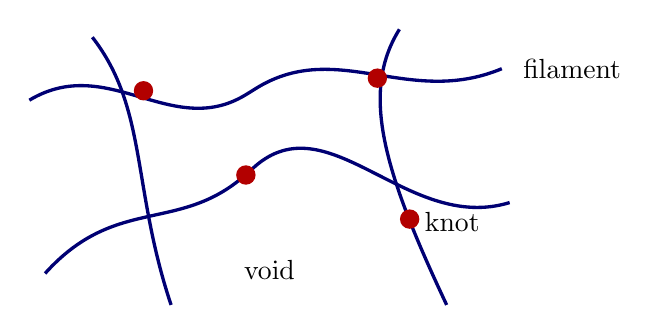
\begin{tikzpicture}[x=1cm,y=1cm]
  \draw[rounded corners=2pt,very thick,blue!45!black]
    (0.2,2.7) .. controls (1.2,3.3) and (2.0,2.2) .. (3.0,2.8)
    .. controls (4.1,3.5) and (5.0,2.6) .. (6.2,3.1);
  \draw[rounded corners=2pt,very thick,blue!45!black]
    (0.4,0.5) .. controls (1.3,1.5) and (2.1,1.0) .. (3.0,1.8)
    .. controls (4.0,2.7) and (5.0,1.0) .. (6.3,1.4);
  \draw[rounded corners=2pt,very thick,blue!45!black]
    (1.0,3.5) .. controls (1.7,2.6) and (1.5,1.6) .. (2.0,0.1);
  \draw[rounded corners=2pt,very thick,blue!45!black]
    (4.9,3.6) .. controls (4.4,2.8) and (4.7,1.8) .. (5.5,0.1);
  \fill[red!70!black] (1.65,2.82) circle (3.5pt);
  \fill[red!70!black] (4.62,2.98) circle (3.5pt);
  \fill[red!70!black] (2.95,1.75) circle (3.5pt);
  \fill[red!70!black] (5.03,1.19) circle (3.5pt);
  \node[align=center] at (3.25,0.55) {void};
  \node[right] at (6.35,3.1) {filament};
  \node[right] at (5.1,1.15) {knot};
\end{tikzpicture}
\caption{Eine klare zweidimensionale Analogie für das Kaustiknetz: Linienförmige Konzentrationen umschließen Voids und treffen an helleren Knoten zusammen. In drei Dimensionen sind die primären Falten Flächen, deren Schnittlinien Filamente und deren Schnittpunkte Knoten bilden.}
\label{fig:c09-caustic-network}
\end{figure}

Die Konstruktion ohne Kräfte ersetzt nicht die kosmologische Störungstheorie. Die Gravitation ist entscheidend für das Anwachsen von Dichtekontrasten, die Entstehung von Halos und Galaxien sowie für die nichtlineare Strukturbildung. Das Spielzeugmodell isoliert eine robuste geometrische Tatsache: Ein anfänglich leicht variierender Fluss faltet sich auf natürliche Weise und erzeugt Konzentrationen. Auch kleine anfängliche Dichtevariationen ließen sich einbeziehen, ohne das zentrale Argument anhand der Jacobi-Determinante zu ändern.

Damit haben wir das Rätsel verlagert, nicht gelöst. Die Inflation wurde eingeführt, um eine Region so stark zu dehnen, dass sie außerordentlich flach und gleichförmig wurde. Die Kaustikrechnung setzt ein anfängliches Feld mit winzigen Geschwindigkeitsvariationen voraus. Woher stammt dieser inhomogene Keim? Die nächste Vorlesung behandelt Quantenfluktuationen der Felder während der Inflation und fragt, wie daraus die Anfangsbedingungen für das spätere kosmische Netz werden.

\section{Was das Argument gezeigt hat}

Ein homogenes Skalarfeld verhält sich wie eine Koordinate, die sich im Potential \(V(\phi)\) bewegt. In einem festen Kasten gilt \(\ddot\phi=-V'(\phi)\). In einem expandierenden komovierenden Kasten geht das physikalische Volumen \(a^3\) in die Wirkung ein und führt zu
\[
\ddot\phi+3H\dot\phi=-V'(\phi).
\]
Die Hubble-Reibung kann das Feld bei einer langsamen Endbewegung auf einem hohen, flachen Potential halten. Dadurch wird seine kinetische Energie vernachlässigbar, seine potentielle Energie hält \(H\) nahezu konstant, und \(a(t)\) wächst annähernd exponentiell.

Die Expansion verdünnt unerwünschte Monopole, glättet die Geometrie und treibt die Krümmung gegen null. Die Inflation muss jedoch enden. Das Feld verlässt das Plateau, oszilliert und überträgt seine Energie auf die heißen Teilchen der Wiederaufheizung. Mehrere Fragen bleiben offen: die Form des Potentials, die Identität und der Anfangszustand des Inflatonfelds, seine Kopplungen bei der Wiederaufheizung und die winzige Vakuumenergie, die heute beobachtet wird.

Der Erfolg der Inflation führt zur abschließenden Frage. Ein vollständig geglättetes Universum enthielte keine Galaxien. Die Kaustikabbildung
\[
y=x+v(x)t,
\qquad
\frac{dn}{dy}=\frac{1}{1+v'(x)t}
\]
zeigt, wie winzige Variationen eines anfänglichen Flusses scharfe Flächen, Filamente und Knoten erzeugen können. Sie erklärt nicht, woher diese Variationen stammen. Nun wenden wir uns ihrem quantenmechanischen Ursprung zu.